\documentclass[conference]{IEEEtran}
\usepackage{graphicx}
\usepackage{booktabs}
\usepackage{amsmath}
\usepackage{array}
\usepackage{url}
\usepackage{tikz}
\usetikzlibrary{positioning,arrows.meta}
\usepackage[hidelinks,pdfauthor={},pdfcreator={},pdftitle={Ground Truth Under Attack: Defending In-Situ Earth-Observation Data Against Valid-Signature False-Data Injection}]{hyperref}
\usepackage{cite}
\usepackage{balance}

\graphicspath{{./}{../../core/docs/figures/}}
\newcommand{\code}[1]{\texttt{\small #1}}

\begin{document}

\title{Ground Truth Under Attack: Defending In-Situ Earth-Observation Data Against Valid-Signature False-Data Injection}

\author{\IEEEauthorblockN{Anonymous Phase~1 Submission}
\IEEEauthorblockA{TSYP14 Technical Challenge, Track~2: False-Data Injection}}

\maketitle

\begin{abstract}
A digital signature proves who sent a sensor reading, not that the reading is true. We present a four-layer
defensive prototype for the in-situ sensing segment of the Earth-observation chain. Layer~1 makes in-transit
and stored-record tampering, replay, deletion and unknown senders deterministically visible with Ed25519
signatures, per-stream sequence numbers and hash chains over mutual-TLS MQTT. Layers~2 and~3 address the
harder case of correctly signed false values: each reading is compared with its own past, two disjoint rings
of neighbours and physical rules, and an Extra Trees classifier per variable turns 37 causal features into a
calibrated p-value and an alert. Layer~4 converts provenance verdicts and alerts into a trust state per
sensor, withholds or imputes suspicious values, and logs every decision in a hash-chained audit trail. On a
full year of real WegenerNet data (2024) with 12 attack families, the frozen detector raises at least one alert on 79--82\,\%
of attacks, while flagging 32--35\,\% of the individual manipulated readings, with 57--60\,\% precision and
0.013 false-alert episodes per stream-day; it doubles F1 over a rule ensemble built from the same signals. A live 30-minute tick for 486
streams takes 0.2\,s on a 2-core CPU with 0.85\,GB peak memory; Ed25519 provenance adds 104 bytes per
record.
\end{abstract}

\begin{IEEEkeywords}
false-data injection, data provenance, anomaly detection, in-situ sensing, Earth observation, Ed25519
\end{IEEEkeywords}

\section{Introduction and Segment Analysis}

Ground stations measuring temperature, relative humidity and precipitation feed frost and drought alerts,
irrigation, parametric insurance and the validation of satellite products. A corrupted observation does not
crash the pipeline: it flows on as a plausible number. Stations are physically exposed, run on low-cost
hardware and are often reached over shared networks, which makes both failure modes of the challenge
realistic: false-data injection and silent failure.

We defend the \emph{in-situ sensing} segment (Track~2) on two axes. \emph{Provenance} establishes who sent a
record and that it was not altered, replayed or dropped. \emph{Plausibility} establishes whether a correctly
signed value is consistent with history, neighbours and physics. Neither is sufficient alone: a compromised
or physically spoofed sensor produces perfectly valid signatures.

Our contributions are: (i)~a threat model separating network/storage attackers from valid-signature
attackers, with an attack taxonomy mapped to the layer expected to catch each family; (ii)~a software
trust anchor with fail-closed verification; (iii)~a causal, calibrated detector evaluated under a strict
chronological protocol with attack families withheld from training; (iv)~a response layer that prevents
suspicious values from reaching the analyst; and (v)~latency, memory and security-overhead measurements on
a laptop CPU.

\section{Related Work}

False-data injection was formalised for power-grid state estimation, where Liu \emph{et al.} showed that an
attacker who knows the system model can inject errors that pass residual-based bad-data checks~\cite{liu-fdi}.
Our setting differs: there is no physical model linking stations, so consistency must be learned from
history and neighbours. Meteorological networks have long used temporal, range and spatial quality-control
tests, such as the spatial regression test of Hubbard \emph{et al.}~\cite{hubbard-qc}; these target sensor
faults, not an adversary who can shape the error. We reuse such tests as features and learn how they combine.
Unsupervised detectors such as Isolation Forest~\cite{iforest} and forecasting models are surveyed
in~\cite{chandola}; in our comparison they react to rare weather and recall few attacks under a strict
false-alarm budget. Our calibration (Eq.~\ref{eq:p}) is a conformal p-value~\cite{vovk}, which makes the
alert threshold a controlled tail probability on clean data. Finally, we report point metrics without point
adjustment, which is known to overstate time-series anomaly detection~\cite{kim-pa}.

\section{Threat Model}

\subsection{Assets and trust boundaries}
Protected assets are measurement values, sensor identities and credentials, freshness and order, processing
evidence and detector inputs, and security decisions. Trusted components are the verifier host, the
provisioned key registry, local policy and state, and the configured trust roots. The trust anchor is in
software (encrypted Ed25519 keys, a local certificate authority, monotonic sequence state), which the
challenge explicitly permits.

\subsection{Attacker classes}
\emph{Network/storage attacker} (no sensor key): modifies, replays, drops, reorders or forges records, or
edits stored readings. Expected catch: Layer~1, deterministic.

\emph{Valid-signature attacker}: controls the reported values of chosen streams over a chosen interval
(compromised sensor or credentials, physical spoofing). The attacker knows the current value, the causal past
and training-period statistics, and may target one site, a neighbourhood of up to 6\,km, or several variables
at once. The attacker cannot alter the evaluator's labels. Expected catch: Layers~2--3, statistical, with
Layer~4 limiting damage.

Out of scope: a compromised verifier host, theft of all trust anchors, unlimited denial of service, and
provable separation of every network fault from an attack.

\begin{table}[t]
\caption{Attack taxonomy and expected catching layer}
\label{tab:taxonomy}
\centering
\small
\begin{tabular}{@{}>{\raggedright}p{0.19\columnwidth}>{\raggedright}p{0.47\columnwidth}>{\raggedright\arraybackslash}p{0.25\columnwidth}@{}}
\toprule
Category & Families & Caught by \\
\midrule
A.~Value, valid signature & bias, drift, spike, noise, flatten, freeze, invalid range, rain scale/suppress/inject,
daily-cycle pattern, mimicry, value replay, coordinated patch, multivariate T+RH, network-wide bias &
L2/L3: temporal, spatial, physical, cross-source \\
B.~Record in transit & tamper value, shift timestamp, replay, drop, reorder & L1: bad signature, replay, gap \\
C.~Stored data & rewrite stored reading, unknown sensor & L1: bad signature, unknown sensor \\
\bottomrule
\end{tabular}
\end{table}

\section{Architecture and Trust Mechanism}

\begin{figure}[t]
\centering
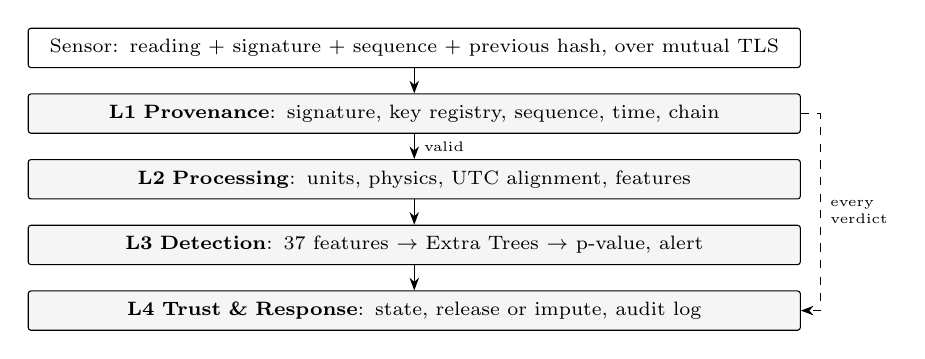
\begin{tikzpicture}[node distance=3.2mm, font=\scriptsize,
  box/.style={draw, rounded corners=1pt, text width=0.80\columnwidth, minimum height=5mm, inner sep=1.5pt, align=center, fill=gray!8},
  >={Stealth[length=1.6mm]}]
\node[box, fill=white] (s) {Sensor: reading + signature + sequence + previous hash, over mutual TLS};
\node[box, below=of s] (l1) {\textbf{L1 Provenance}: signature, key registry, sequence, time, chain};
\node[box, below=of l1] (l2) {\textbf{L2 Processing}: units, physics, UTC alignment, features};
\node[box, below=of l2] (l3) {\textbf{L3 Detection}: 37 features $\rightarrow$ Extra Trees $\rightarrow$ p-value, alert};
\node[box, below=of l3] (l4) {\textbf{L4 Trust \& Response}: state, release or impute, audit log};
\draw[->] (s) -- (l1); \draw[->] (l1) -- node[right, font=\tiny]{valid} (l2); \draw[->] (l2) -- (l3); \draw[->] (l3) -- (l4);
\draw[->, dashed] (l1.east) -- ++(2.5mm,0) |- node[pos=0.25, right, font=\tiny, align=left]{every\\verdict} (l4.east);
\end{tikzpicture}
\caption{The four layers run in one Python process on a laptop. Every Layer~1 verdict, including rejections,
also reaches Layer~4, so failures are never silent.}
\label{fig:arch}
\end{figure}

Fig.~\ref{fig:arch} shows the pipeline. Layers exchange typed, immutable contracts with generated JSON
schemas.

\subsection{Layer 1: provenance}
Each sensor holds its own Ed25519~\cite{ed25519} key, encrypted at rest. A reading is encoded in canonical CBOR with a
per-stream sequence number and the hash of the previous record, then signed. The signer commits sequence
allocation, chain advance and the exact signed bytes atomically to a durable outbox \emph{before}
publishing, so a crash never reuses a sequence number. Transport is MQTT~v5 over mutual TLS only, with
per-sensor topic ACLs; transport security is independent of the signature. A persistent verifier checks the
signature, key-registry entry (enrolment, rotation, revocation), sequence, time window and chain, and
returns an explicit status (\code{valid}, \code{bad\_signature}, \code{replay}, \code{gap},
\code{chain\_anomaly}, \code{unknown\_sensor}, \code{malformed}). Authentication failure never advances
state. A software anchor can be defeated by an administrator restoring an old database; no hardware
anti-rollback is claimed.

\subsection{Layer 4: trust and response}
Every 30 minutes each sensor is \emph{trusted}, \emph{suspicious} ($\geq 3$ alerted ticks in 6\,h) or
\emph{quarantined} ($\geq 6$ in 12\,h, or $\geq 3$ provenance failures in 2\,h). Suspicious and quarantined
values are imputed from the median of at least two trusted neighbours, or withheld. A single forged message
never quarantines a sensor, since otherwise anyone could silence a sensor without its key; it is flagged,
audited and never released. Provenance quarantine ends only by an analyst release recorded with name and
reason. Thresholds were set by Monte-Carlo simulation on the detector's measured behaviour, assuming each attacked
tick alerts independently with probability 0.33 (the measured reading recall): 0.072 false quarantines per
sensor-month, while every simulated 24--48\,h attack is quarantined (median 8\,h). Real alerts cluster in
time, so these figures are indicative. Decisions
go to an append-only SQLite log with its own SHA-256 chain; triggers reject updates and deletions. A
FastAPI dashboard shows states, raw versus released values and chain status.

\section{Signal Processing}

Layer~2 uses only provenance-valid readings for statistics and never modifies raw signed evidence. It
normalises units (\textdegree C/\textdegree F/K with absolute-zero limits), checks physical ranges, aligns
readings to exact UTC windows with explicit missingness, and emits feature windows with rolling statistics,
conditional spectral features (only when sampling supports them) and neighbour comparisons. Event time and
availability time are kept separate so no replay can use future data.

The detector computes 37 features per reading, each using only values up to time $t$ (unit-tested: changing
a future value never changes an earlier feature). Rain is modelled as $\log(1+x)$; scales are robust
($1.4826\cdot$MAD) per site and variable.
\begin{itemize}
\item \emph{Temporal (11)}: residual to a forecast $b\,x_{t-1}+(1-b)\,x_{t-48}$, residual to a per-site
harmonic seasonal model, a two-sided CUSUM~\cite{cusum} that accumulates slow drifts, 3\,h and 24\,h median, MAD
and standard deviation, and 3\,h slope.
\item \emph{Spatial (14)}: residuals to a distance-weighted median of a \emph{near ring} (6 closest sites)
and a disjoint \emph{wider ring} (19th--24th closest), with weights capped at 45\,\% so one attacked
neighbour cannot dominate; neighbour spread, count and co-movement.
\item \emph{Physical rules (4)}: range violation, rate of change, freeze run length (exempt for dry rain and
saturated humidity) and variability ratio.
\item \emph{Context (8)}: hour and day of year, rain occurrence and amount, value and quality flag.
\end{itemize}
The disjoint wider ring answers coordinated attacks that corrupt the near neighbours; CUSUM answers drifts
that never produce a single large step.

\section{Detector Design and Evaluation}

\subsection{Model, calibration and alert rule}
One Extra Trees~\cite{extratrees} classifier per variable (120 trees, depth $\leq 18$) learns which combinations of signals
indicate manipulation; for example, a deviation from the past together with moving neighbours is weather,
not an attack. It was the strongest of 11 candidates under the same false-alarm budget; GRU/TCN forecasters,
a sequence autoencoder and Isolation Forest react to any unusual weather and recall few attacks under a strict
budget. Training replays each 14-day episode clean and with four seeded attacked copies; a quarter of the
clean samples are hard cases with large genuine neighbour residuals. Scores are calibrated on clean data as
\begin{equation}
p = \frac{1 + \#\{\text{clean scores} \geq s\}}{n + 1},
\label{eq:p}
\end{equation}
so one budget applies to all variables. Per variable, an alert is raised when $p \leq \alpha$, directly or
with two-of-three confirmation, choosing the best F1 subject to $\leq 0.05$ false-alert episodes per
stream-day and $\geq 95\,\%$ coverage. The rule is then frozen together with the SHA-256 of every model file;
the detector refuses to run if any file changes.

\subsection{Data and protocol}
We use WegenerNet Level~2 v8.0 (University of Graz, CC~BY~4.0)~\cite{wegenernet}, half-hourly 100\,m grid,
Feldbach region, 2023--2024. A 1.5\,km sub-grid of cells clean for $\geq 95\,\%$ of training gives 162 sites
$\times$ 3 variables $=$ 486 streams. Splits are strictly chronological: Jan--Aug 2023 training, Sep--Oct
calibration, Nov--Dec rule selection, and 2024 for evaluation only. Metrics are strict point metrics without
point adjustment, plus event detection (at least one alert during the attack).

\subsection{Results}

\begin{table}[t]
\caption{Frozen detector on 2024 (two attack seeds)}
\label{tab:results}
\centering
\small
\setlength{\tabcolsep}{3.5pt}
\begin{tabular}{@{}lccccc@{}}
\toprule
 & Prec. & Rec. & F1 & Events & FA/sd \\
\midrule
Seed 91000 & 57.1\,\% & 31.8\,\% & 0.408 & 79.2\,\% & 0.013 \\
Seed 191000 & 59.6\,\% & 35.3\,\% & 0.443 & 82.2\,\% & 0.013 \\
Rule ensemble & 31.8\,\% & 17--18\,\% & 0.22--0.23 & 51--55\,\% & 0.046 \\
\bottomrule
\end{tabular}

\vspace{2pt}
\footnotesize Rec.: recall over attacked readings. Events: share of attacks with at least one alert.
FA/sd: false-alert episodes per stream-day on clean 2024 (budget 0.05).
\end{table}

Table~\ref{tab:results} reports the results. Coverage is 100\,\%. The gap between attacks detected (about four
in five) and readings flagged (about one in three) is expected: an alert early in an attack is enough to act on,
but the readings before evidence accumulates, such as the first steps of a slow drift, are missed. The false-alarm rate corresponds to about
one false episode per stream every 2.5 months, four times under the budget. Against a rule ensemble fusing
the same temporal, spatial and physical scores with an Isolation Forest, the learned detector roughly doubles
precision, recall and F1 and produces 3.5$\times$ fewer false alarms (Fig.~\ref{fig:vsrules}).

\begin{figure}[t]
\centering
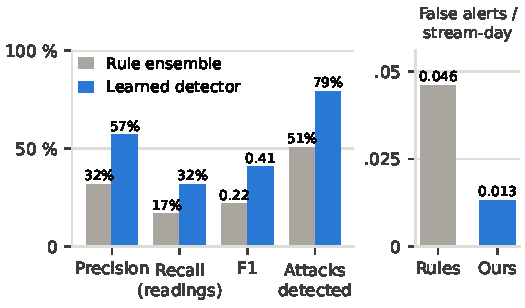
\includegraphics[width=\columnwidth]{fig_detector_vs_rules.pdf}
\caption{Learned detector versus rule ensemble on the same signals (2024, seed 91000).}
\label{fig:vsrules}
\end{figure}

Per family (Fig.~\ref{fig:families}), invalid range and freeze are always detected through the physical
rules; noise and flatten (93--96\,\% of attacks), bias (85--93\,\%) and drift (78--93\,\%) are detected as
events, though not every manipulated reading inside them.

\begin{figure}[t]
\centering
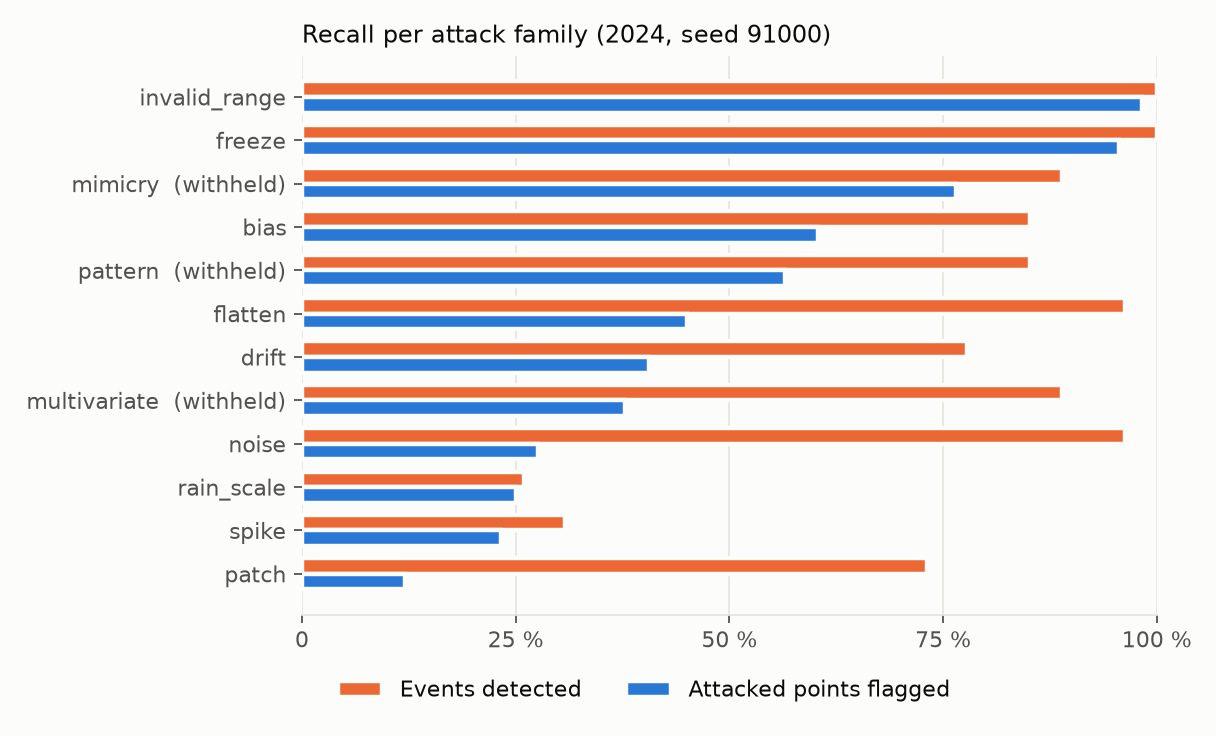
\includegraphics[width=0.92\columnwidth]{family_recall.png}
\caption{Detection per attack family (2024, seed 91000). Families marked withheld were never seen in
training.}
\label{fig:families}
\end{figure}

\section{Standard Scenario and Evasion}

\subsection{Scenario}
The standard scenario is versioned and seeded, and built on real public data;
rebuilds are byte-identical (SHA-256 manifests) and the jury can re-run it with its own held-out attacks. It
has two parts: (i)~the detector protocol above, with one non-overlapping attack per family per 14-day episode,
6--48\,h long, and two independent 2024 seeds; (ii)~a station suite on 154 WegenerNet 5-minute stations with 16
value families plus record and storage faults, split into \emph{dev} (108 stations), \emph{heldout} (46
different stations, different sizes, two held-out-only shapes), \emph{clean2024} for false alarms and
\emph{crosssource} for whole-network bias.

\subsection{Evasion}
Table~\ref{tab:evasion} summarises how an informed attacker might evade detection and what happens.

\begin{table}[t]
\caption{Evasion strategies and outcomes}
\label{tab:evasion}
\centering
\small
\begin{tabular}{@{}>{\raggedright}p{0.25\columnwidth}>{\raggedright\arraybackslash}p{0.69\columnwidth}@{}}
\toprule
Strategy & Outcome \\
\midrule
Unseen attack types & withheld from training: pattern 81--85\,\%, mimicry 89--100\,\%, multivariate 89--96\,\% detected \\
Different magnitudes & 2024: $\pm$0.75, 1.5, 3\,\textdegree C; training: $\pm$0.5, 1, 2, 4\,\textdegree C (inside the range: interpolation) \\
Match own statistics & mimicry with training mean/variance: 89--100\,\% detected, spatially \\
Hide in the daily cycle & pattern: 81--85\,\% detected \\
Corrupt neighbours & patch up to 6\,km: 69--73\,\% detected via the wider ring \\
Shift whole network$^\dagger$ & neighbours blind ($<2\,\%$ alarms); cross-source baseline alarms on ${\sim}100\,\%$ of cells \\
Stay below threshold$^\dagger$ & escape sweep (rule baseline): largest size still missed per family \\
Forge or replay records & Layer~1 rejects 100/100 tampered records, audited \\
\bottomrule
\end{tabular}

\vspace{2pt}
\footnotesize $^\dagger$Station suite, rule-based baselines (unit test and \code{eval/escape.py}); the trained
detector is graded on it in Phase~2.
\end{table}

\subsection{Limitations}
Single-step spikes carry little evidence (23--48\,\% of readings). Rain scaling is hard (14--25\,\% of
readings): about 90\,\% of intervals are dry and only 773 attacked rain rows exist for training. A coordinated
regional shift is not separable from real weather using in-situ data alone; this is where the remote-sensing
input is required, through a cross-source check against ERA5-Land~\cite{era5land}. Grading the trained detector
on the station suite and adding the cross-source reference are the main Phase~2 extensions. The 2024 attacks
share their generator with training (with new placements, interpolated sizes and three withheld families), so the figures are strong
evidence rather than an independent benchmark.

\section{Feasibility and Local Execution}

\begin{table}[t]
\caption{Cost on a 2-core x86-64 CPU (no GPU, no cloud)}
\label{tab:cost}
\centering
\small
\begin{tabular}{@{}p{0.54\columnwidth}p{0.40\columnwidth}@{}}
\toprule
Measurement & Value \\
\midrule
Live tick (486 streams, 24\,h history) & median 202\,ms; p95 236\,ms \\
Share of the 30-min interval used & $<0.02\,\%$ used \\
Batch replay, 14 days & 5.0\,s (16.5\,\textmu s/reading) \\
Detector peak memory / model size & 852\,MB / 17.6\,MB \\
Ed25519 sign / verify (incl.\ chain) & 17\,700 / 8\,050 rec./s, one core \\
Overhead per record & 104\,B (64 sig.\ + 8 seq.\ + 32 hash) \\
Tampered rejected / false rejections & 100/100, 0 \\
\bottomrule
\end{tabular}
\end{table}

Table~\ref{tab:cost} summarises cost. All rows were measured on the same 2-core x86-64 machine, with the
shipped artifacts (outputs in \code{reports/detector-overhead.json} and \code{reports/crypto-benchmark.json}); latency depends on array shape and model, not on values, so the measurement needs no data
download. No purchase, GPU, cloud service or paid API is required, and dependencies are hash-locked.

\section{Reproducibility}

The test suite (745 passed, 17 skipped; skipped tests need a local broker; log in
\code{reports/test-results.txt}) includes no-look-ahead and
label-leakage tests for the detector. The frozen model ships with SHA-256 hashes; one command reproduces
Table~\ref{tab:results} from the public data and another retrains from scratch. A jury guide documents
installation, data download, every command and how to read each output, and a command-line tool lets the jury
plant its own attack and inspect the detector's p-values and alerts. Detector latency and memory are
reproduced with \code{python -m eval.detector\_overhead}.

\section{Conclusion}

Signatures and plausibility checks are complementary: Layer~1 makes record-level attacks deterministic, and
the calibrated detector raises an alert on about four out of five valid-signature attacks at a low
false-alarm rate, including attack families it never saw, although it flags only about one in three
manipulated readings and slow drifts are caught late. Layer~4 ensures that what the detector misses or
flags does not silently reach the analyst. The remaining blind spot, coordinated regional bias, is exactly the
case that requires combining in-situ data with remote-sensing references, which is the focus of Phase~2.


\begin{thebibliography}{1}
\bibitem{wegenernet}
J.~Fuchsberger, G.~Kirchengast, C.~Bichler, \emph{et al.}, ``WegenerNet climate station network Level~2 data
version~8.0 (2007--2024),'' Wegener Center for Climate and Global Change, Univ.\ of Graz, 2025,
doi:~10.25364/WEGC/WPS8.0-2025.1.
\bibitem{era5land}
J.~Mu\~noz-Sabater \emph{et al.}, ``ERA5-Land: A state-of-the-art global reanalysis dataset for land
applications,'' \emph{Earth Syst.\ Sci.\ Data}, vol.~13, no.~9, pp.~4349--4383, 2021.
\bibitem{ed25519}
D.~J.~Bernstein, N.~Duif, T.~Lange, P.~Schwabe, and B.-Y.~Yang, ``High-speed high-security signatures,''
\emph{J.\ Cryptogr.\ Eng.}, vol.~2, no.~2, pp.~77--89, 2012.
\bibitem{extratrees}
P.~Geurts, D.~Ernst, and L.~Wehenkel, ``Extremely randomized trees,'' \emph{Mach.\ Learn.}, vol.~63, no.~1,
pp.~3--42, 2006.
\bibitem{cusum}
E.~S.~Page, ``Continuous inspection schemes,'' \emph{Biometrika}, vol.~41, no.~1/2, pp.~100--115, 1954.
\bibitem{liu-fdi}
Y.~Liu, P.~Ning, and M.~K.~Reiter, ``False data injection attacks against state estimation in electric power
grids,'' in \emph{Proc.\ 16th ACM Conf.\ Computer and Communications Security (CCS)}, 2009, pp.~21--32.
\bibitem{hubbard-qc}
K.~G.~Hubbard, S.~Goddard, W.~D.~Sorensen, N.~Wells, and T.~T.~Osugi, ``Performance of quality assurance
procedures for an applied climate information system,'' \emph{J.\ Atmos.\ Oceanic Technol.}, vol.~22, no.~1,
pp.~105--112, 2005.
\bibitem{iforest}
F.~T.~Liu, K.~M.~Ting, and Z.-H.~Zhou, ``Isolation forest,'' in \emph{Proc.\ IEEE Int.\ Conf.\ Data Mining
(ICDM)}, 2008, pp.~413--422.
\bibitem{chandola}
V.~Chandola, A.~Banerjee, and V.~Kumar, ``Anomaly detection: A survey,'' \emph{ACM Comput.\ Surv.}, vol.~41,
no.~3, art.~15, 2009.
\bibitem{vovk}
V.~Vovk, A.~Gammerman, and G.~Shafer, \emph{Algorithmic Learning in a Random World}. New York, NY, USA:
Springer, 2005.
\bibitem{kim-pa}
S.~Kim, K.~Choi, H.-S.~Choi, B.~Lee, and S.~Yoon, ``Towards a rigorous evaluation of time-series anomaly
detection,'' in \emph{Proc.\ AAAI Conf.\ Artificial Intelligence}, 2022, pp.~7194--7201.
\end{thebibliography}

\end{document}
